% outlines.tex
%
% written 2022 by Werner Lemberg <wl@gnu.org>


% This file contains graphics used for the 'FreeType Glyph Conventions'
% tutorial, part 6, 'FreeType Outlines'.


% Here is one possibility to convert this LaTeX file to both PNG and SVG
% formats.
%
%   xelatex outlines.tex
%
%   pdftoppm -png -f 1 -l 6 -r 120 outlines.pdf outlines
%   optipng outlines-*.png
%
%   for i in 1 2 3 4 5 6; do
%     pdf2svg outlines.pdf outlines-$i.svg $i
%   done


\documentclass[tikz, border=3mm]{standalone}

\usepackage{libertinus}

\usetikzlibrary{
  calc,
  decorations,
  fit,
  positioning
}

% We need exact bounding boxes.
\usepgflibrary{bbox}


% Node styles.
\tikzset{
  % For second-order Bézier curves.
  conic/.style={
    to path={(\tikztostart)
               .. controls ($#1!1/3!(\tikztostart)$)
                  and ($#1!1/3!(\tikztotarget)$)
               .. (\tikztotarget)}},
%
  % For virtual on-points.
  hollow square/.style={
    line width=1pt,
    draw,
    fill=white,
    minimum size=6pt,
    inner sep=0pt,
    outer sep=0pt},
%
  % For on-points.
  filled square/.style={
    fill,
    minimum size=6pt,
    inner sep=0pt,
    outer sep=0pt},
%
  % 'Elastic dashes' adapt spaces between dashes to the line length so that
  % the last dash doesn't get cut off partially.
  %
  % Taken from
  % https://tex.stackexchange.com/questions/133271/can-tikz-dashed-lines-emulate-pstricks-dashed-lines
  elastic dash/.code args={on #1 off #2}{
    % Use csname so catcode of @ doesn't have do be changed.
    \csname tikz@addoption\endcsname{%
      \pgfgetpath\currentpath
      \pgfprocessround{\currentpath}{\currentpath}%
      \csname pgf@decorate@parsesoftpath\endcsname
        {\currentpath}{\currentpath}%
      \pgfmathparse{\csname pgf@decorate@totalpathlength\endcsname-#1}%
      \let\rest=\pgfmathresult
      \pgfmathparse{#1+#2}%
      \let\onoff=\pgfmathresult
      \pgfmathparse{max(floor(\rest/\onoff), 1)}%
      \let\nfullonoff=\pgfmathresult
      \pgfmathparse{max((\rest-\onoff*\nfullonoff)/\nfullonoff+#2, #2)}%
      \let\offexpand=\pgfmathresult
      \pgfsetdash{{#1}{\offexpand}}{0pt}}},
%
  % For main curves.
  line/.style={
    line width=2pt},
%
  % For auxiliary, dashed curves.
  dashed line/.style={
    elastic dash=on 6pt off 6pt,
    line width=1pt},
  % For auxiliary, densely dashed curves.
  densely dashed line/.style={
    elastic dash=on 3pt off 3pt,
    line width=1pt,
    line cap=rect},
%
  % For off-points.
  hollow dot/.style={
    draw,
    line width=1pt,
    circle,
    minimum size=6pt,
    inner sep=0pt},
%
  % For explanations.
  description/.style={
    font=\Large\itshape},
}


%%%%%%%%%%%%%%%%%%%%%%%%%%%%%%%%%%%%%%%%%%%%%%%%%%%%%%%%%%%%%%%%%%%%%%%%%%%%%

\begin{document}

% It looks better for the curves to start and end at the center of the
% nodes, avoiding a little bit of unwanted whitespace next to the on-point
% boxes.

% A line segment.

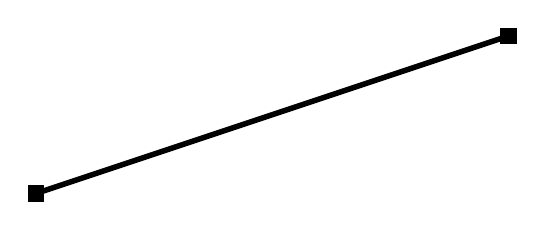
\begin{tikzpicture}
  \node[filled square] (A) at (0,0) {};
  \node[filled square] (B) at (6,2) {};

  \draw[line] (A.center) -- (B.center);
\end{tikzpicture}


% A conic curve with one off-point.

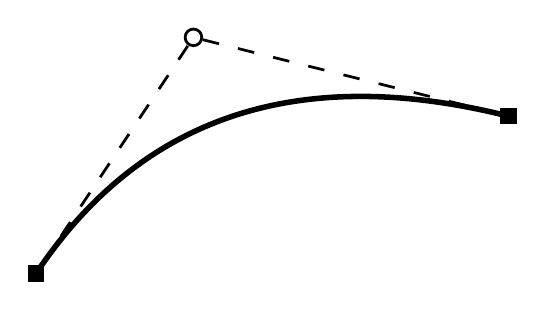
\begin{tikzpicture}
  \node[filled square] (A) at (0,0) {};
  \node[hollow dot] (B) at (2,3) {};
  \node[filled square] (C) at (6,2) {};

  \draw[dashed line] (A) -- (B);
  \draw[dashed line] (B) -- (C);

  \draw[line] (A.center) to[conic={(B)}] (C.center);
\end{tikzpicture}


% A cubic curve with two off-points.

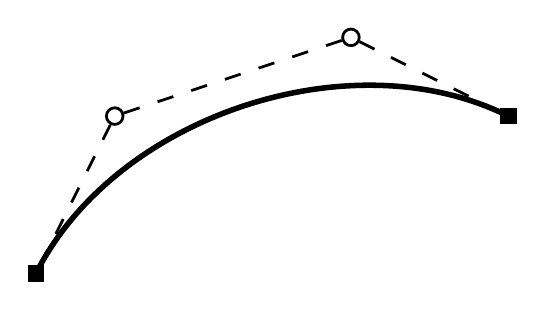
\begin{tikzpicture}
  \node[filled square] (A) at (0,0) {};
  \node[hollow dot] (B) at (1,2) {};
  \node[hollow dot] (C) at (4,3) {};
  \node[filled square] (D) at (6,2) {};

  \draw[dashed line] (A) -- (B);
  \draw[dashed line] (B) -- (C);
  \draw[dashed line] (C) -- (D);

  \draw[line] (A.center) .. controls (B) and (C) .. (D.center);
\end{tikzpicture}


% A conic curve with two off-points and virtual on-point inbetween.

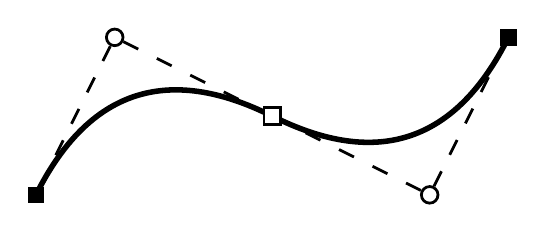
\begin{tikzpicture}
  \node[filled square] (A) at (0,0) {};
  \node[hollow dot] (B) at (1,2) {};
  \node[hollow dot] (D) at (5,0) {};
  \node[filled square] (E) at (6,2) {};

  \coordinate (C) at ($ (B) !.5! (D) $);

  \draw[dashed line] (A) -- (B);
  \draw[dashed line] (B) -- (C);
  \draw[dashed line] (C) -- (D);
  \draw[dashed line] (D) -- (E);

  \draw[line] (A.center) to[conic={(B)}] (C.center);
  \draw[line] (C.center) to[conic={(D)}] (E.center);

  % This comes last since it must white out the inner part of the box.
  \node[hollow square] at (C) {};
\end{tikzpicture}


% Show that the bounding box (bbox) can differ from the control point
% bounding box (cbox).

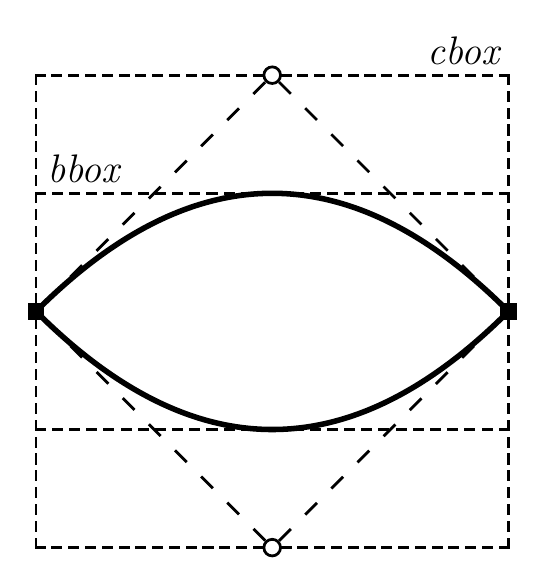
\begin{tikzpicture}[bezier bounding box]
  \coordinate (A) at (0,0);
  \coordinate (B) at (3,3);
  \coordinate (B') at (3,-3);
  \coordinate (C) at (6,0);

  \path[save path=\pathtop] (A.center) to[conic={(B)}] (C.center);
  \path[save path=\pathbottom] (A.center) to[conic={(B')}] (C.center);

  \node[fit=(current bounding box),
        inner sep=0pt,
        outer sep=0pt] (bbox) {};

  \node[filled square] (A) at (A) {};
  \node[hollow dot] (B) at (B) {};
  \node[hollow dot] (B') at (B') {};
  \node[filled square] (C) at (C) {};

  \draw[dashed line] (A) -- (B);
  \draw[dashed line] (B) -- (C);
  \draw[dashed line] (A) -- (B');
  \draw[dashed line] (B') -- (C);

  \draw[line] [use path=\pathtop];
  \draw[line] [use path=\pathbottom];

  \draw[densely dashed line] (A) -- (A |- B);
  \draw[densely dashed line] (A |- B) -- (B);
  \draw[densely dashed line] (B) -- (B -| C)
    node[description, pos=0.8, above] {cbox};
  \draw[densely dashed line] (B -| C) -- (C);

  \draw[densely dashed line] (A) -- (A |- B');
  \draw[densely dashed line] (A |- B') -- (B');
  \draw[densely dashed line] (B') -- (B' -| C);
  \draw[densely dashed line] (B' -| C) -- (C);

  \draw[densely dashed line] (bbox.north west) -- (bbox.north east)
    node[description, pos=0.1, above] {bbox};
  \draw[densely dashed line] (bbox.south west) -- (bbox.south east);
\end{tikzpicture}


% Show that the bounding box (bbox) is identical to the control point
% bounding box (cbox) if the curve uses points at the extrema.

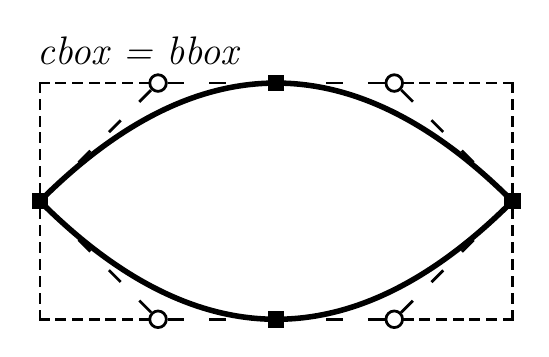
\begin{tikzpicture}
  \coordinate (P) at (3,3);
  \coordinate (P') at (3,-3);

  \node[filled square] (A) at (0,0) {};
  \node[filled square] (E) at (6,0) {};

  \node[hollow dot] (B) at ($ (A) !.5! (P) $) {};
  \node[hollow dot] (D) at ($ (P) !.5! (E) $) {};
  \node[filled square] (C) at ($ (B) !.5! (D) $) {};

  \node[hollow dot] (B') at ($ (A) !.5! (P') $) {};
  \node[hollow dot] (D') at ($ (P') !.5! (E) $) {};
  \node[filled square] (C') at ($ (B') !.5! (D') $) {};

  % It looks better for these two curves to start and end at the center of
  % the nodes, avoiding a little bit of unwanted whitespace next to the
  % on-point boxes.
  \draw[line] (A.center) to[conic={(B)}] (C.center);
  \draw[line] (C.center) to[conic={(D)}] (E.center);
  \draw[line] (A.center) to[conic={(B')}] (C'.center);
  \draw[line] (C'.center) to[conic={(D')}] (E.center);

  \draw[dashed line] (A) -- (B);
  \draw[dashed line] (B) -- (C);
  \draw[dashed line] (C) -- (D);
  \draw[dashed line] (D) -- (E);

  \draw[dashed line] (A) -- (B');
  \draw[dashed line] (B') -- (C');
  \draw[dashed line] (C') -- (D');
  \draw[dashed line] (D') -- (E);

  \draw[densely dashed line] (A) -- (A |- B);
  \draw[densely dashed line] (A |- B) -- (B)
    node[description, pos=0.9, above, yshift=1mm] {cbox = bbox};
  \draw[densely dashed line] (D) -- (D -| E);
  \draw[densely dashed line] (D -| E) -- (E);

  \draw[densely dashed line] (A) -- (A |- B');
  \draw[densely dashed line] (A |- B') -- (B');
  \draw[densely dashed line] (D') -- (D' -| E);
  \draw[densely dashed line] (D' -| E) -- (E);
\end{tikzpicture}

\end{document}
